\documentclass[conference,onecolumn]{IEEEtran}

\usepackage[T1]{fontenc}
\usepackage[utf8]{inputenc}
\usepackage[spanish,es-tabla]{babel}
\usepackage{lmodern}
\usepackage{microtype}
\usepackage{csquotes}
\usepackage{amsmath,amssymb}
\usepackage{booktabs}
\usepackage{float}
\usepackage{tabularx}
\usepackage{array}
\usepackage{longtable}
\usepackage{graphicx}
\usepackage{url}
\usepackage[hidelinks]{hyperref}
\usepackage[backend=biber,style=ieee,sorting=none]{biblatex}
\addbibresource{referencias.bib}
\AtBeginDocument{\spanishplainpercent}

\newcolumntype{Y}{>{\raggedright\arraybackslash}X}
\newcolumntype{L}[1]{>{\raggedright\arraybackslash}p{#1}}
\renewcommand{\IEEEkeywordsname}{Palabras clave}

\title{TA-IND-01: ISO/IEC/IEEE 29148 y tipos de requisitos de Apple Music}
\author{\IEEEauthorblockN{Danela Dayana Arteaga Alava}\IEEEauthorblockA{Carrera de Software\\
Facultad de Ciencias de la Computación\\
Universidad Técnica Estatal de Quevedo, Ecuador\\
Ingeniería de Requerimientos -- ISR-401}}

\begin{document}
\maketitle

\begin{abstract}
Trabajo individual que aplica la norma ISO/IEC/IEEE 29148:2018 a Apple Music, un sistema de uso frecuente por la autora. Incluye la descripción del sistema, un resumen analítico de la norma, un glosario, la formulación y clasificación de 15 requisitos con sus criterios de aceptación, la autoevaluación de cada requisito y una reflexión final.
\end{abstract}

\begin{IEEEkeywords}
Ingeniería de requisitos, ISO/IEC/IEEE 29148:2018, ISO/IEC 25010:2023, tipos de requisitos, Apple Music.
\end{IEEEkeywords}

\section*{Datos generales}

\begin{table}[H]
\centering\footnotesize
\begin{tabularx}{\textwidth}{@{}p{0.22\textwidth}Y@{}}
\toprule
\textbf{Campo} & \textbf{Detalle}\\
\midrule
Asignatura & Ingeniería de Requerimientos (ISR-401) · 4.\textsuperscript{o} nivel · Paralelo B\\
Estudiante & Arteaga Alava Danela Dayana\\
Docente & Gleiston Cicerón Guerrero Ulloa, PhD\\
Sistema analizado & Apple Music\\
Fecha de cierre & Sábado 7 de noviembre de 2026, 23:59\\
Repositorio & \url{https://github.com/darteagaa-boop/ISR401-ArteagaDanela}\\
\bottomrule
\end{tabularx}
\end{table}

\section{Descripción del sistema}
Apple Music es un servicio de música por suscripción de Apple que permite escuchar canciones en streaming, guardarlas en una biblioteca personal, crear listas de reproducción y descargarlas para escucharlas sin conexión. Funciona en la aplicación para iPhone, en computadoras y desde el navegador, y también tiene aplicación para Android.

Utilizo Apple Music casi todos los días desde mi celular para escuchar música mientras realizo mis actividades diarias, estudio o cuando estoy haciendo las tareas del hogar. Lo uso principalmente para buscar mis canciones favoritas, crear listas de reproducción y escuchar música. También aprovecho la opción de descargar canciones para escucharlas cuando no tengo conexión a internet, esta opción me sirve mucho cuando tengo un viaje largo.

Las funciones principales que se analizan son la búsqueda en el catálogo, biblioteca y listas de reproducción, descargas sin conexión, letras sincronizadas, sincronización entre dispositivos y gestión de la suscripción.

\section{Capturas del sistema}

\begin{figure}[H]
\centering
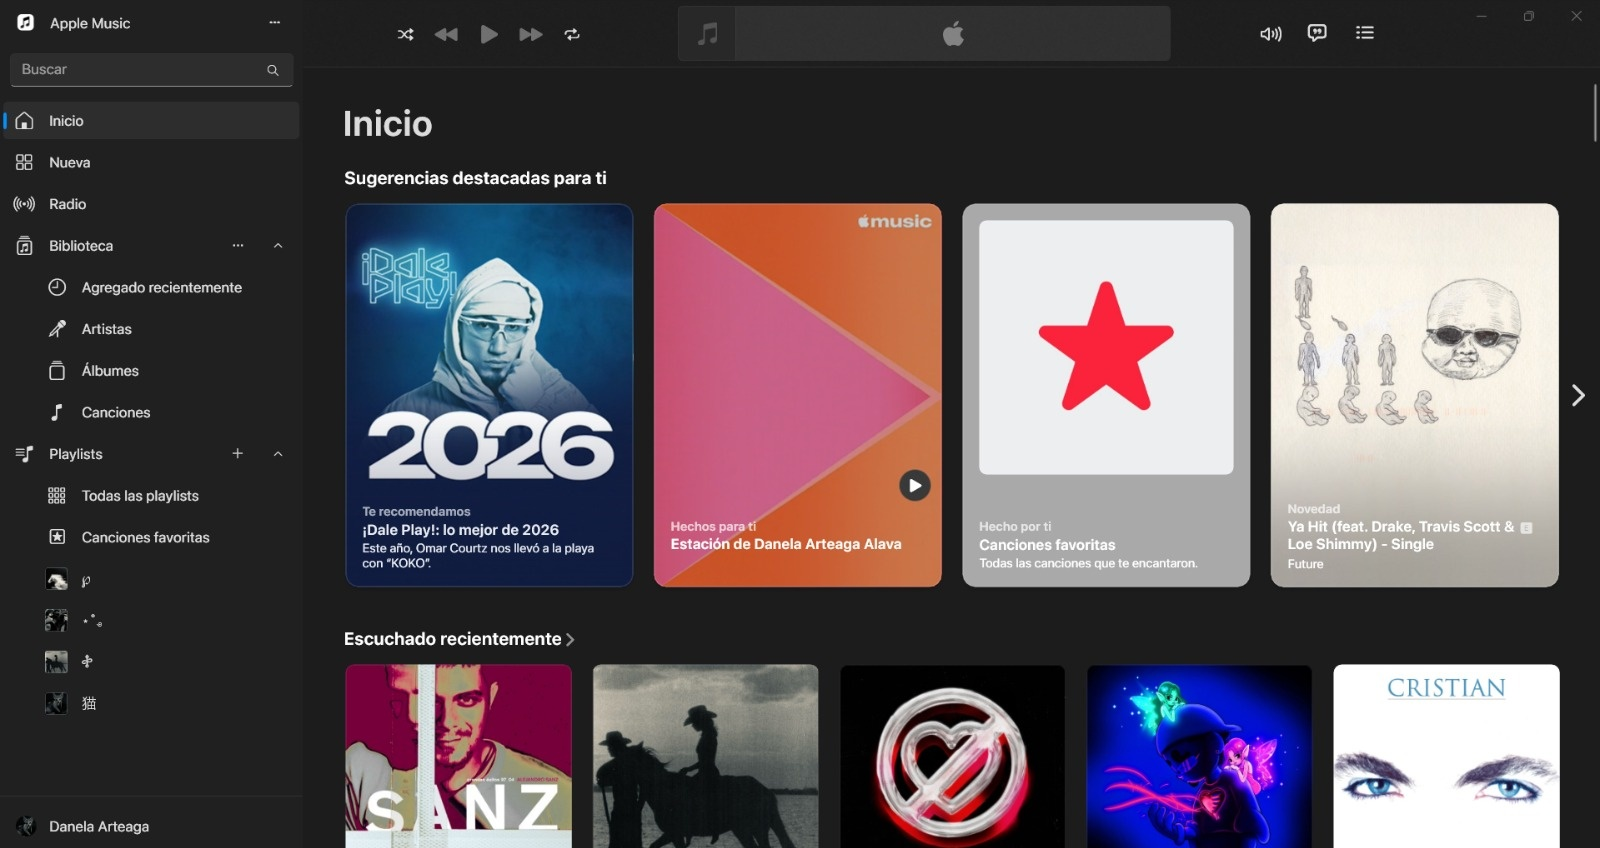
\includegraphics[width=0.75\textwidth]{figuras/captura-inicio.jpg}
\caption{Pantalla de inicio de Apple Music. Fuente: captura propia.}
\label{fig:inicio}
\end{figure}

\begin{figure}[H]
\centering
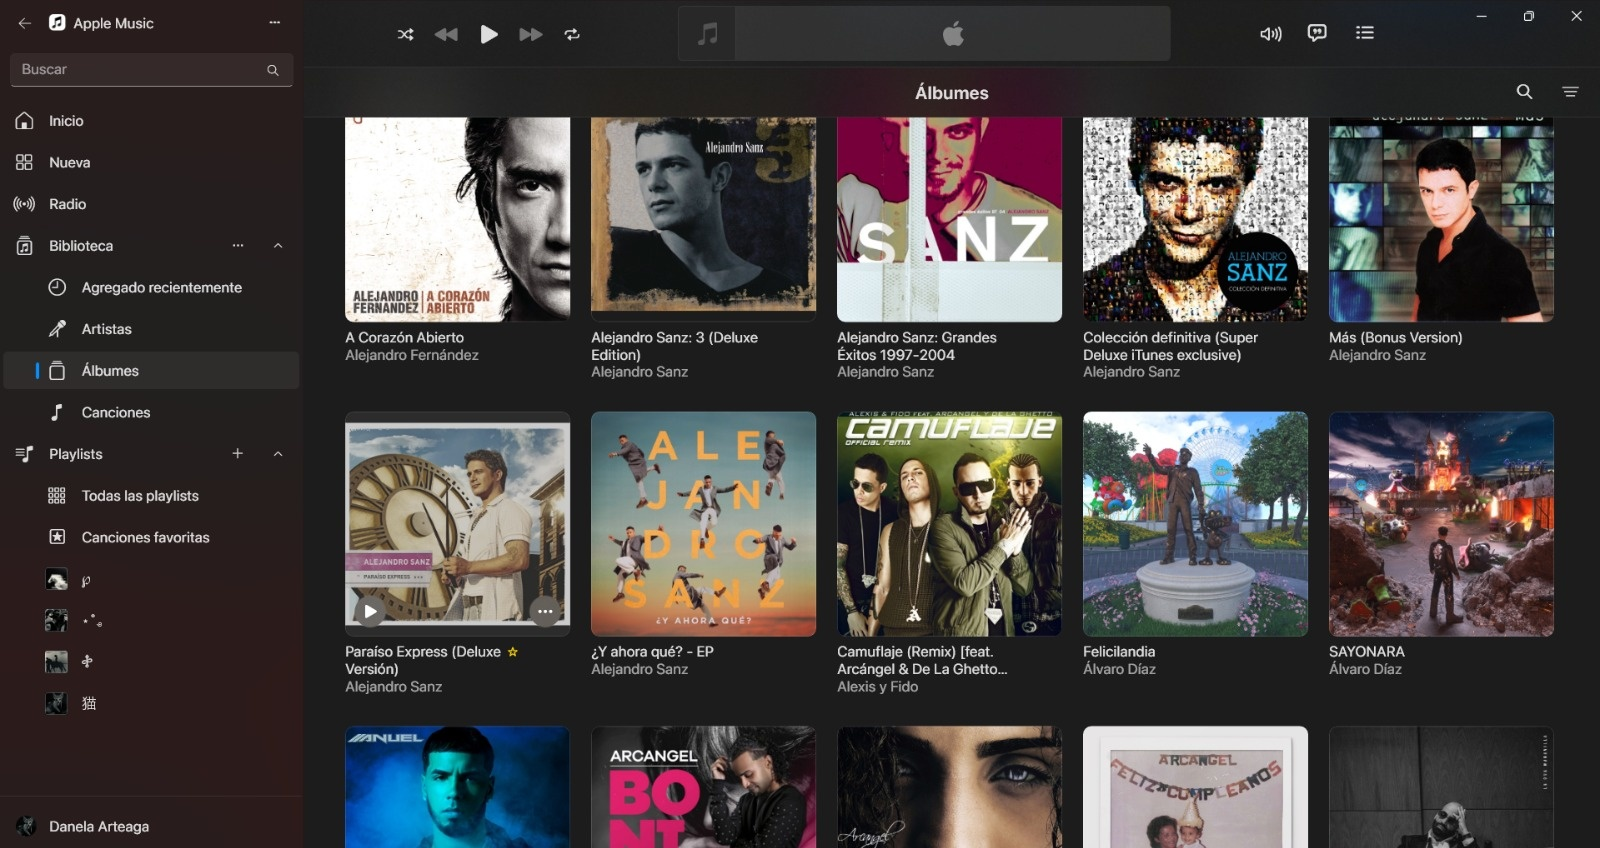
\includegraphics[width=0.75\textwidth]{figuras/captura-biblioteca.jpg}
\caption{Biblioteca de Apple Music con álbumes y listas de reproducción. Fuente: captura propia.}
\label{fig:biblioteca}
\end{figure}

\begin{figure}[H]
\centering
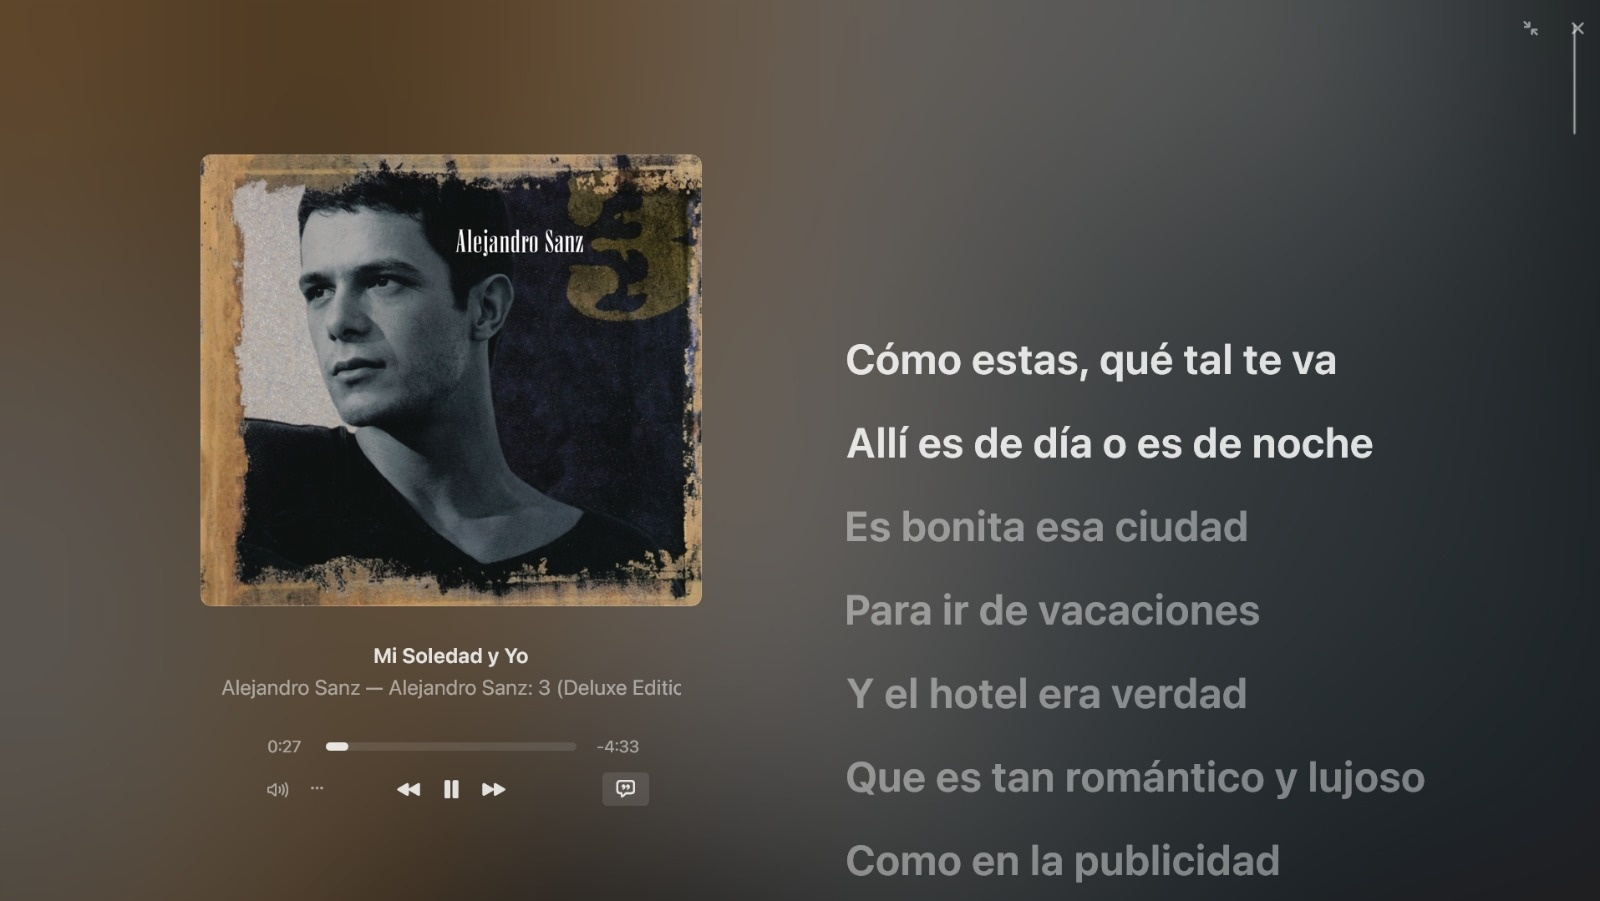
\includegraphics[width=0.75\textwidth]{figuras/captura-reproductor.jpg}
\caption{Reproductor de Apple Music con la letra sincronizada. Fuente: captura propia.}
\label{fig:reproductor}
\end{figure}

\section{Requisitos de Apple Music y tabla de clasificación}
Se formulan 15 requisitos de seis tipos distintos, de cuales los seis requisitos de calidad se clasifican con ISO/IEC 25010:2023 \cite{iso25010} y se cuantifican con métrica y umbral, agregando de que cada requisito incluye su criterio de aceptación.

{\footnotesize
\setlength{\tabcolsep}{3pt}
\begin{longtable}{@{}L{0.04\textwidth}L{0.33\textwidth}L{0.10\textwidth}L{0.15\textwidth}L{0.33\textwidth}@{}}
\caption{Requisitos de Apple Music, clasificación y criterios de aceptación}\label{tab:requisitos}\\
\toprule
\textbf{ID} & \textbf{Requisito} & \textbf{Tipo} & \textbf{Característica ISO/IEC 25010:2023} & \textbf{Criterio de aceptación}\\
\midrule
\endfirsthead
\toprule
\textbf{ID} & \textbf{Requisito} & \textbf{Tipo} & \textbf{Característica ISO/IEC 25010:2023} & \textbf{Criterio de aceptación}\\
\midrule
\endhead
\midrule
\multicolumn{5}{r@{}}{\emph{Continúa en la página siguiente}}\\
\endfoot
\bottomrule
\endlastfoot
R01 & El sistema deberá permitir al usuario buscar canciones, álbumes, artistas y listas de reproducción escribiendo texto en el buscador. & Funcional & - & Se acepta si, al escribir el nombre de un artista, álbum o canción existente en el catálogo, este aparece entre los resultados.\\
R02 & El sistema deberá permitir al usuario crear, renombrar y eliminar listas de reproducción en su biblioteca. & Funcional & - & Se acepta si el usuario puede crear una lista, cambiarle el nombre y eliminarla, y cada cambio se refleja en su biblioteca.\\
R03 & El sistema deberá permitir descargar canciones de la biblioteca para reproducirlas sin conexión a internet mientras la suscripción esté activa. & Funcional & - & Se acepta si una canción descargada se reproduce completa con el modo avión activado.\\
R04 & El sistema deberá mostrar la letra de la canción en reproducción, sincronizada con el audio, siempre y cuando la letra esté disponible. & Funcional & - & Se acepta si, en una canción con letra disponible, la línea resaltada coincide con la parte que se está escuchando.\\
R05 & La reproducción en streaming de una canción deberá iniciar en 2 segundos o menos en el 95 \% de los casos, con una conexión de 10 Mbps o superior. & Calidad & Eficiencia de desempeño, comportamiento temporal & Se acepta si, en 100 reproducciones medidas con una conexión de 10 Mbps, al menos 95 inician en 2 s o menos.\\
R06 & El servicio de streaming deberá estar disponible al menos el 99,9 \% del tiempo de cada mes. & Calidad & Fiabilidad, disponibilidad & Se acepta si el monitoreo mensual registra 43 minutos o menos de caída del servicio.\\
R07 & El 100 \% de los datos de la cuenta y de pago deberá transmitirse cifrado con TLS 1.2 o superior. & Calidad & Seguridad, confidencialidad & Se acepta si al revisar el tráfico de la aplicación no se encuentra ninguna conexión sin cifrar que envíe datos de la cuenta o de pago.\\
R08 & Los cambios en la biblioteca hechos en un dispositivo deberán aparecer en los demás dispositivos de la misma cuenta en 60 segundos o menos en el 95 \% de los casos. & Calidad & Compatibilidad, interoperabilidad & Se acepta si, en 20 pruebas de agregar una canción en el teléfono, al menos 19 aparecen en la computadora en 60 s o menos.\\
R09 & Al menos el 90 \% de los usuarios nuevos deberá poder crear una lista de reproducción y agregarle 3 canciones en 2 minutos o menos, sin ayuda. & Calidad & Capacidad de interacción, aprendibilidad & Se acepta si, en una prueba con al menos 10 usuarios nuevos, 9 o más completan la tarea en 2 min o menos.\\
R10 & Durante la reproducción continua con la pantalla apagada, la aplicación no deberá consumir más del 5 \% de la batería por hora. & Calidad & Eficiencia de desempeño, utilización de recursos & Se acepta si, tras 1 hora de reproducción con la pantalla apagada, la batería del teléfono de prueba baja 5 \% o menos.\\
R11 & El sistema deberá permitir controlar reproducir, pausar, siguiente y anterior desde la pantalla de bloqueo y desde auriculares Bluetooth. & Interfaz externa & - & Se acepta si las cuatro acciones funcionan desde la pantalla de bloqueo y desde los botones de unos auriculares Bluetooth.\\
R12 & La aplicación móvil deberá funcionar en teléfonos con iOS 17 o superior y con Android 10 o superior. & Restricción técnica & - & Se acepta si la aplicación se instala y reproduce música en un teléfono con iOS 17 y en uno con Android 10.\\
R13 & El sistema deberá impedir que las canciones descargadas se reproduzcan fuera de la aplicación o después de cancelar la suscripción, para respetar las licencias de derechos de autor. & Legal & - & Se acepta si, tras cancelar la suscripción, las canciones descargadas dejan de reproducirse y los archivos no se abren en otro reproductor.\\
R14 & El tratamiento de los datos personales de los usuarios en Ecuador deberá cumplir la Ley Orgánica de Protección de Datos Personales \cite{lopdp2021}. & Legal & - & Se acepta si el usuario puede consultar, corregir y eliminar sus datos personales desde la configuración de su cuenta, y existe una política de privacidad publicada.\\
R15 & El sistema deberá permitir el acceso al catálogo completo solo a usuarios con una suscripción activa. & Regla de negocio & - & Se acepta si una cuenta sin suscripción no puede reproducir canciones completas del catálogo y una cuenta con suscripción sí puede.\\
\end{longtable}
}

{\footnotesize
\setlength{\tabcolsep}{3pt}
\begin{longtable}{@{}L{0.25\textwidth}L{0.45\textwidth}L{0.15\textwidth}@{}}
\caption{Resumen de requisitos por tipo}\label{tab:resumen}\\
\toprule
\textbf{Tipo} & \textbf{Requisitos} & \textbf{Cantidad}\\
\midrule
\endfirsthead
\toprule
\textbf{Tipo} & \textbf{Requisitos} & \textbf{Cantidad}\\
\midrule
\endhead
\midrule
\multicolumn{3}{r@{}}{\emph{Continúa en la página siguiente}}\\
\endfoot
\bottomrule
\endlastfoot
Funcional & R01, R02, R03, R04 & 4\\
Calidad & R05, R06, R07, R08, R09, R10 & 6\\
Interfaz externa & R11 & 1\\
Restricción técnica & R12 & 1\\
Legal & R13, R14 & 2\\
Regla de negocio & R15 & 1\\
Total & 6 tipos distintos & 15\\
\end{longtable}
}

\printbibliography[title={Referencias}]
\end{document}
